%%% Preamble
\documentclass{report}

\usepackage[utf8]{inputenc}
\usepackage[T1]{fontenc}
\usepackage{fourier}
\usepackage[french]{babel}
\usepackage[protrusion=true,expansion=true]{microtype}	
\usepackage{amsmath,amsfonts,amsthm} % Math packages
\usepackage[pdftex]{graphicx}	
\usepackage{url}
\usepackage{pdfpages}
\usepackage{todonotes}
\usepackage[a4paper, body={16cm,26cm}]{geometry}
\usepackage{float}
\usepackage{framed}
\usepackage[toc,page]{appendix} 
\usepackage{multicol}
\usepackage{colortbl}
\usepackage{epstopdf}
\usepackage{adjustbox}

%%% Custom sectioning
\usepackage{sectsty}
\allsectionsfont{  \normalfont\scshape}
%\allsectionsfont{\centering \normalfont\scshape}

%%% Custom headers/footers (fancyhdr package)
\usepackage{fancyhdr}
\pagestyle{fancyplain}
\fancyhead{}								% No page header
\fancyfoot[L]{}							% Empty 
\fancyfoot[C]{}							% Empty
\fancyfoot[R]{\thepage}					% Pagenumbering
\renewcommand{\headrulewidth}{0pt}		% Remove header underlines
\renewcommand{\footrulewidth}{0pt}		% Remove footer underlines
\setlength{\headheight}{13.6pt}


%%% Equation and float numbering
\numberwithin{equation}{section}		% Equationnumbering: section.eq#
\numberwithin{figure}{section}		% Figurenumbering: section.fig#
\numberwithin{table}{section}		% Tablenumbering: section.tab#


%%% Define new commands
\newcommand{\horrule}[1]{\rule{\linewidth}{#1}} 	% Horizontal rule
\renewcommand{\bf}[1]{\textbf{#1}}
\renewcommand{\it}[1]{\textit{#1}}
\newcommand{\bfit}[1]{\textbf{\textit{#1}}}
\renewcommand{\sc}[1]{\textsc{#1}}

\newcommand{\Todo}[1]{\todo[inline]{#1}}
\renewcommand{\thesection}{\thepart .\arabic{section}}

\usepackage{tocloft}
\cftsetindents{chapter}{0em}{1em}
\cftsetindents{section}{1.5em}{2.5em}
\makeatletter
\def\l@figure{\@dottedtocline{1}{1.5em}{4em}}
\makeatother

\usepackage{bookmark}
%\usepackage[hidelinks]{hyperref}
\usepackage{cases}
\usepackage{color}
\usepackage{xcolor}
\usepackage{relsize}
\usepackage{caption}
\colorlet{shadecolor}{black!10}

\delimitershortfall-1sp
\newcommand\abs[1]{\left|#1\right|}


\usepackage{tikz, pgfplots}


%}}}
%{{{ --- pgfplots ---------------------

%{{{ Colors

% TolColors from http://www.r-bloggers.com/the-paul-tol-21-color-salute/
\definecolor{TolColor1}{HTML}{332288}   % dark purple
\definecolor{TolColor2}{HTML}{6699CC}   % dark blue
\definecolor{TolColor3}{HTML}{88CCEE}   % light blue
\definecolor{TolColor4}{HTML}{44AA99}   % light green
\definecolor{TolColor5}{HTML}{117733}   % dark green
\definecolor{TolColor6}{HTML}{999933}   % dark brown
\definecolor{TolColor7}{HTML}{DDCC77}   % light brown
\definecolor{TolColor8}{HTML}{661100}   % dark red
\definecolor{TolColor9}{HTML}{CC6677}   % light red
\definecolor{TolColor10}{HTML}{AA4466}  % light pink
\definecolor{TolColor11}{HTML}{882255}  % dark pink
\definecolor{TolColor12}{HTML}{AA4499}  % light purple

%}}}
%{{{ Color cycles

\pgfplotscreateplotcyclelist{mbarplot cycle}{%
  {draw=TolColor2, fill=TolColor2!70},
  {draw=TolColor7, fill=TolColor7!70},
  {draw=TolColor4, fill=TolColor4!70},
  {draw=TolColor11, fill=TolColor11!70},
  {draw=TolColor1, fill=TolColor1!70},
  {draw=TolColor8, fill=TolColor8!70},
  {draw=TolColor6, fill=TolColor6!70},
  {draw=TolColor9, fill=TolColor9!70},
  {draw=TolColor10, fill=TolColor10!70},
  {draw=TolColor12, fill=TolColor12!70},
  {draw=TolColor3, fill=TolColor3!70},
  {draw=TolColor5, fill=TolColor5!70},
}

\pgfplotscreateplotcyclelist{mlineplot cycle}{%
  {TolColor2, mark=*, mark size=1.5pt},
  {TolColor7, mark=square*, mark size=1.3pt},
  {TolColor4, mark=triangle*, mark size=1.5pt},
  {TolColor6, mark=diamond*, mark size=1.5pt},
}


\pgfplotsset{
  compat=1.9,
  mbaseplot/.style={
    legend style={
      draw=none,
      fill=none,
      cells={anchor=west},
    },
    x tick label style={
      font=\footnotesize
    },
    y tick label style={
      font=\footnotesize
    },
    legend style={
      font=\footnotesize
    },
    major grid style={
      dotted,
    },
    axis x line*=bottom,
  },
  mlineplot/.style={
    mbaseplot,
    xmajorgrids=true,
    ymajorgrids=true,
    major grid style={dotted},
    axis x line=bottom,
    axis y line=left,
    legend style={
      cells={anchor=west},
      draw=none
    },
    cycle list name=mlineplot cycle,
  },
  mbarplot base/.style={
    mbaseplot,
    bar width=6pt,
    axis y line*=none,
  },
  mbarplot/.style={
    mbarplot base,
    ybar,
    xmajorgrids=false,
    ymajorgrids=true,
    area legend,
    legend image code/.code={%
      \draw[#1] (0cm,-0.1cm) rectangle (0.15cm,0.1cm);
    },
    cycle list name=mbarplot cycle,
  },
  horizontal mbarplot/.style={
    mbarplot base,
    xmajorgrids=true,
    ymajorgrids=false,
    xbar stacked,
    area legend,
    legend image code/.code={%
      \draw[#1] (0cm,-0.1cm) rectangle (0.15cm,0.1cm);
    },
    cycle list name=mbarplot cycle,
  },
  disable thousands separator/.style={
    /pgf/number format/.cd,
      1000 sep={}
  },
}


%%  ========   IMPORTANT ========
%% Spécifier ici les variables pour le document
\newcommand{\mainTitle}{\'Etude préalable - SPIE}
\newcommand{\secondTitle}{Dossier d'évaluation des solutions}
\newcommand{\documentRef}{DC/4401/1}
\newcommand{\auteurs}{
Lisa \textsc{Courant} \\
Estelle \textsc{Lepeigneux} \\
Pierre \textsc{Jarsaillon} \\
Hugues \textsc{Verlin} \\
}
\newcommand{\chefDeProjet}{Paul \textsc{Dautry}}
\newcommand{\responsableQualite}{Antoine \textsc{Chabert}}

%%% Begin document
\begin{document}
%----------------------------------------------------------------------------------------
%	PACKAGES
%----------------------------------------------------------------------------------------

\documentclass[12pt]{article}
\usepackage[a4paper]{geometry}
\geometry{verbose,tmargin=1in,bmargin=0in,lmargin=1in,rmargin=1in}
\usepackage[utf8]{inputenc}
\usepackage[francais]{babel}
\usepackage[T1]{fontenc}

\usepackage{graphicx}
\begin{document}

\begin{titlepage}

\newcommand{\HRule}{\rule{\linewidth}{0.5mm}} % horizontal lines

\center % Center everything
 
%----------------------------------------------------------------------------------------
%	HEADING SECTIONS
%----------------------------------------------------------------------------------------

\vspace*{1cm}

\textsc{\LARGE INSA de LYON}\\[1.5cm] 
\textsc{\Large D\'epartement Informatique}\\[0.5cm] 
\textsc{\large Projet Longue Durée}\\[0.5cm] % 

%----------------------------------------------------------------------------------------
%	TITLE SECTION
%----------------------------------------------------------------------------------------

\HRule \\[0.4cm]
{ \huge \bfseries Compte Rendu}\\[0.1cm]
{\large \bfseries - Gestion des contacts commerciaux d'une banque -} 
\HRule \\[1.5cm]
 
%----------------------------------------------------------------------------------------
%	DATE SECTION
%----------------------------------------------------------------------------------------

{\large \today}\\[2cm] % 
 
%----------------------------------------------------------------------------------------
%	AUTHOR SECTION
%----------------------------------------------------------------------------------------

\begin{minipage}{0.4\textwidth}
\begin{center} \large
\emph{Auteurs} \\
Lisa \textsc{Courant} \\
Estelle \textsc{Lepeigneux} \\
Pierre \textsc{Jarsaillon} \\
Hugues \textsc{Verlin} \\
\end{center}
\end{minipage}
~
\begin{minipage}{0.4\textwidth}
\begin{center} \large
\emph{Chef de projet} \\
Paul \textsc{Dautry}
\end{center}
\begin{center} \large
\emph{Responsable Qualité} \\
Antoine \textsc{Chabert}
\end{center}
\end{minipage}\\[5cm]

H4401\\[2cm]

%----------------------------------------------------------------------------------------
%	LOGO SECTION
%----------------------------------------------------------------------------------------

\includegraphics[scale=0.3]{figures/logo.png}
%----------------------------------------------------------------------------------------

\vfill % Fill the rest of the page with whitespace

\end{titlepage}
\end{document}


%% Commenter les deux lignes suivantes pour le document final
\listoftodos
\newpage

%% Table de matière / figures / tableaux
\tableofcontents
\listoffigures
\listoftables
\newpage

%% Faire une nouvelle partie :
\part{Solution Standard}
\setcounter{section}{0}
\section{Rappel des fonctionnalités de la solution informatique et organisationnelle}

Une solution standard est une solution qui s’appuie sur les bonnes pratiques recommandées par un éditeur de progiciel de gestion intégré. L’information est mise à jour en temps réel dans l’ensemble des modules associés au module qui vient d’être modifié, et il est aisé de retrouver l’origine de chaque information. Cette solution peut couvrir l’ensemble du SI d’une entreprise, ou bien seulement une partie si l’on choisit de n’implémenter que certains modules de SAP. \\

Pour SPIE, nous avons choisi l’ERP SAP, et celui-ci couvrira l’ensemble du SI lié aux métiers de la maintenance. Le choix de cette solution permettrait d’homogénéiser le SI de SPIE avec un outil unique couvrant un très large périmètre de gestion. La découpe en modules fonctionnels permet une personnalisation maximale, chacun couvrant un des périmètres de l’entreprise.

\section{Chiffrages des coûts (d'acquisition et de possession)}

\begin{shaded}
\noindent\textsc{Note :} 

Voir Annexe A pour le tableau d'évaluation.
\end{shaded}

Il y a deux types de coûts : les coûts d’acquisition et les coûts de possession. Les premiers ne seront investis qu’une seule et unique fois par l’entreprise, tandis que les seconds permettent le fonctionnement de la société et permettent d’exploiter les biens acquis précédemment. \\

En faisant le choix d’une solution standard, appuyée sur SAP, les coûts d’acquisition sont assez minimes. En effet, les investissements sur cette solution sont peu portées sur les immobilisations corporelles, telles les tablettes tactiles, mais plus sur un coût de formation SAP, délivré aux employés de SPIE Sud-Est. \\

Cependant, si l’investissement initial est peu élevé, la majorité des coûts de la solution standard seront répartis dans le temps. En effet, SAP By Design fonctionne sur un système d’abonnement : pour chaque utilisateur, et chaque année, un abonnement de 1 596 euros doit être payé. Certains services sont également payant, proportionnellement au prix de l’abonnement, par un ratio de 1. Étant donné le nombre important d’utilisateurs de la solution, soit 300 techniciens et 20 utilisateurs sur site, il est compréhensible que les coûts montent rapidement. En revanche, les coûts de maintenance, liés à l’investissement initial correspondant à un pourcentage de ce dernier, ne représentent pas un important montant annuel. La deuxième source de coût de possession correspond aux salaires des nouveaux poste de travail suggérés pour superviser les nouveaux équipements proposés.


\begin{figure}[H]
    \noindent\makebox[\textwidth]{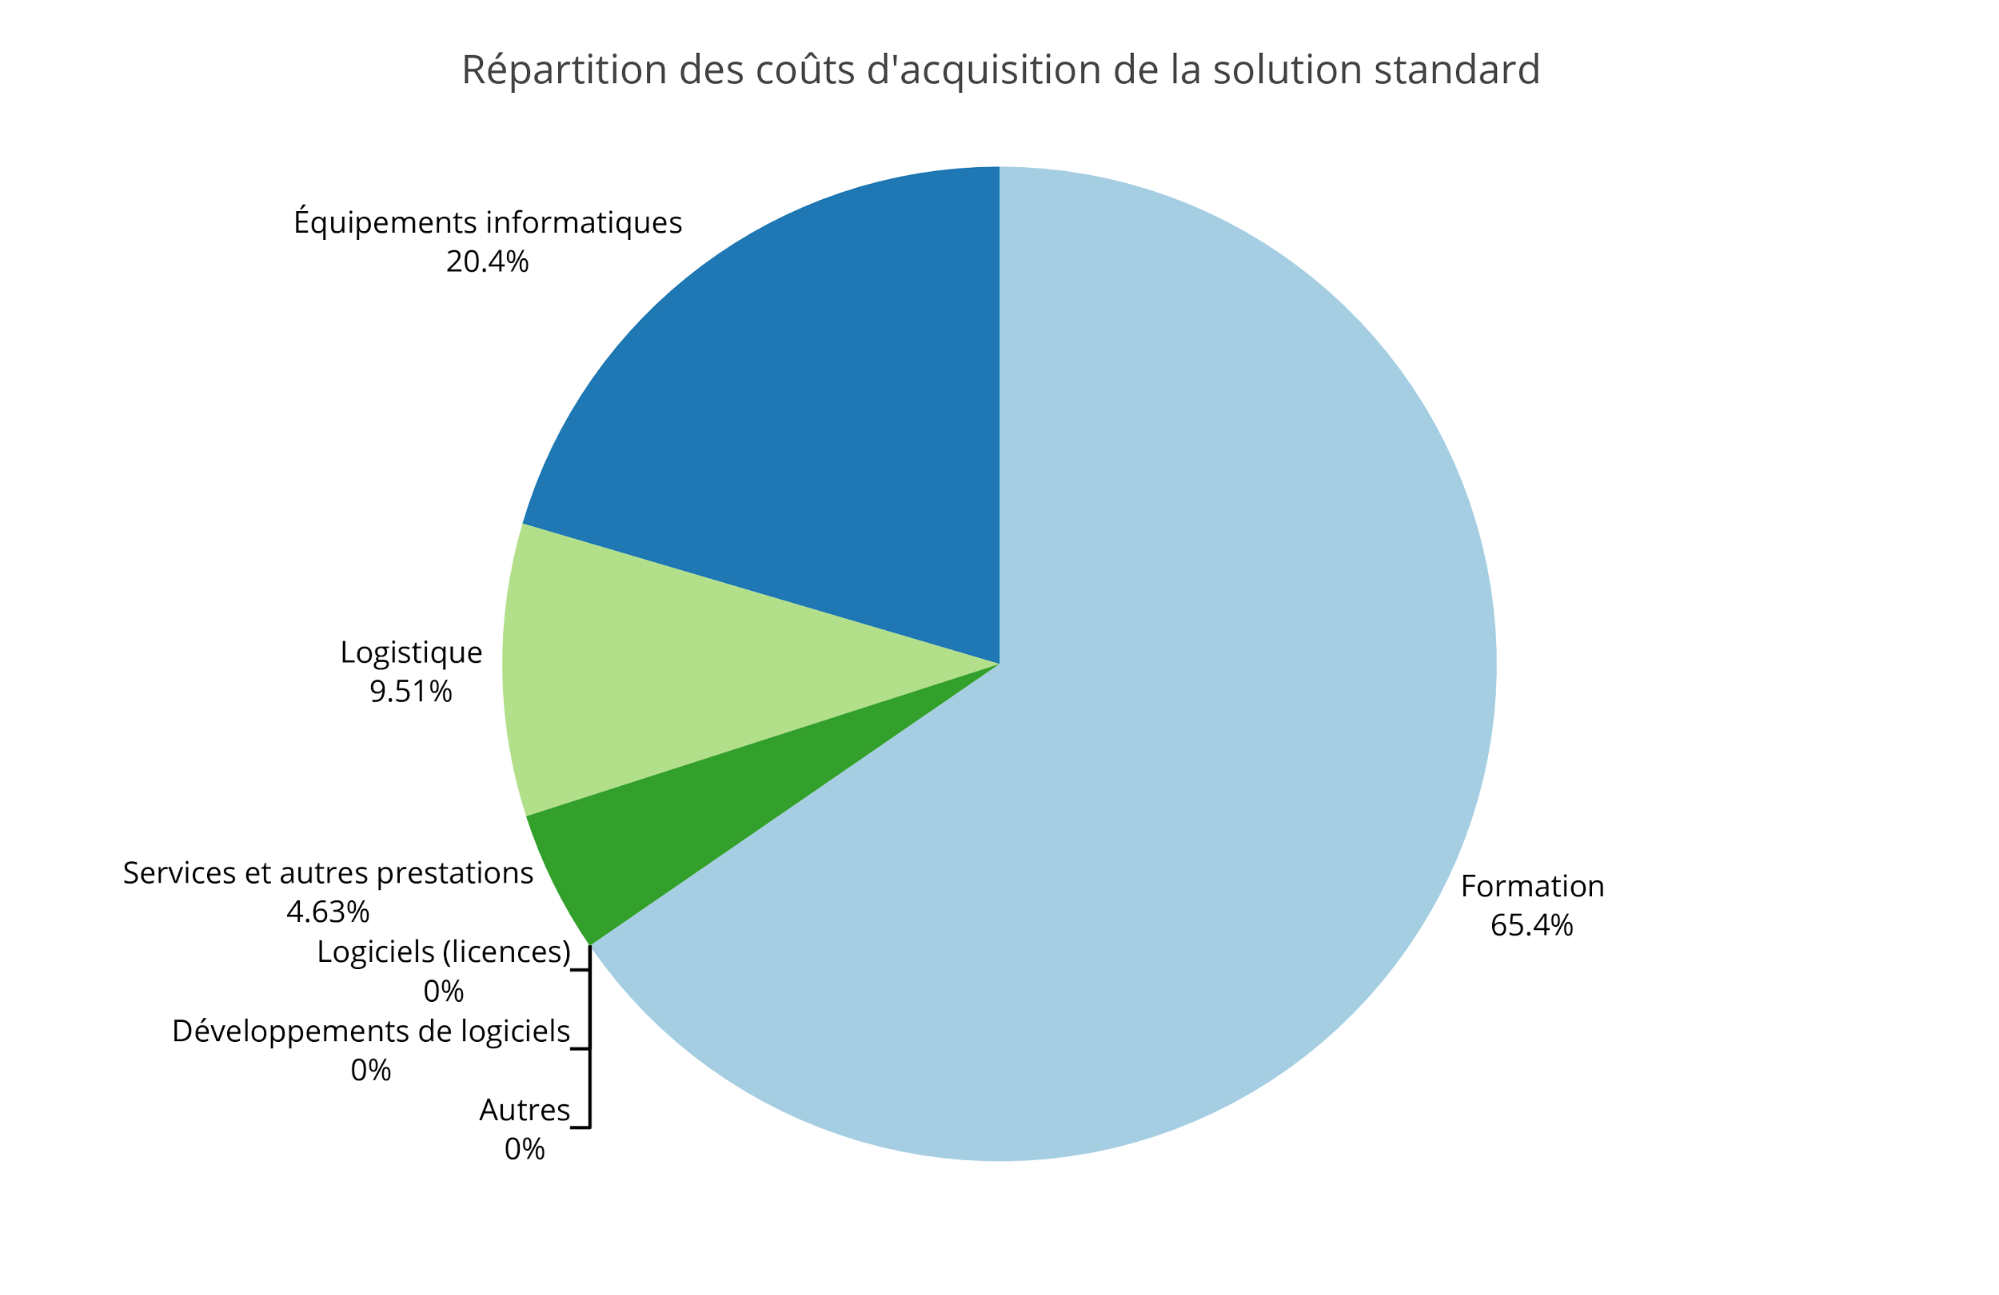
\includegraphics[width=12cm]{figures/cout_acquisition_sol_standard.png}}
\end{figure}

\begin{figure}[H]
    \noindent\makebox[\textwidth]{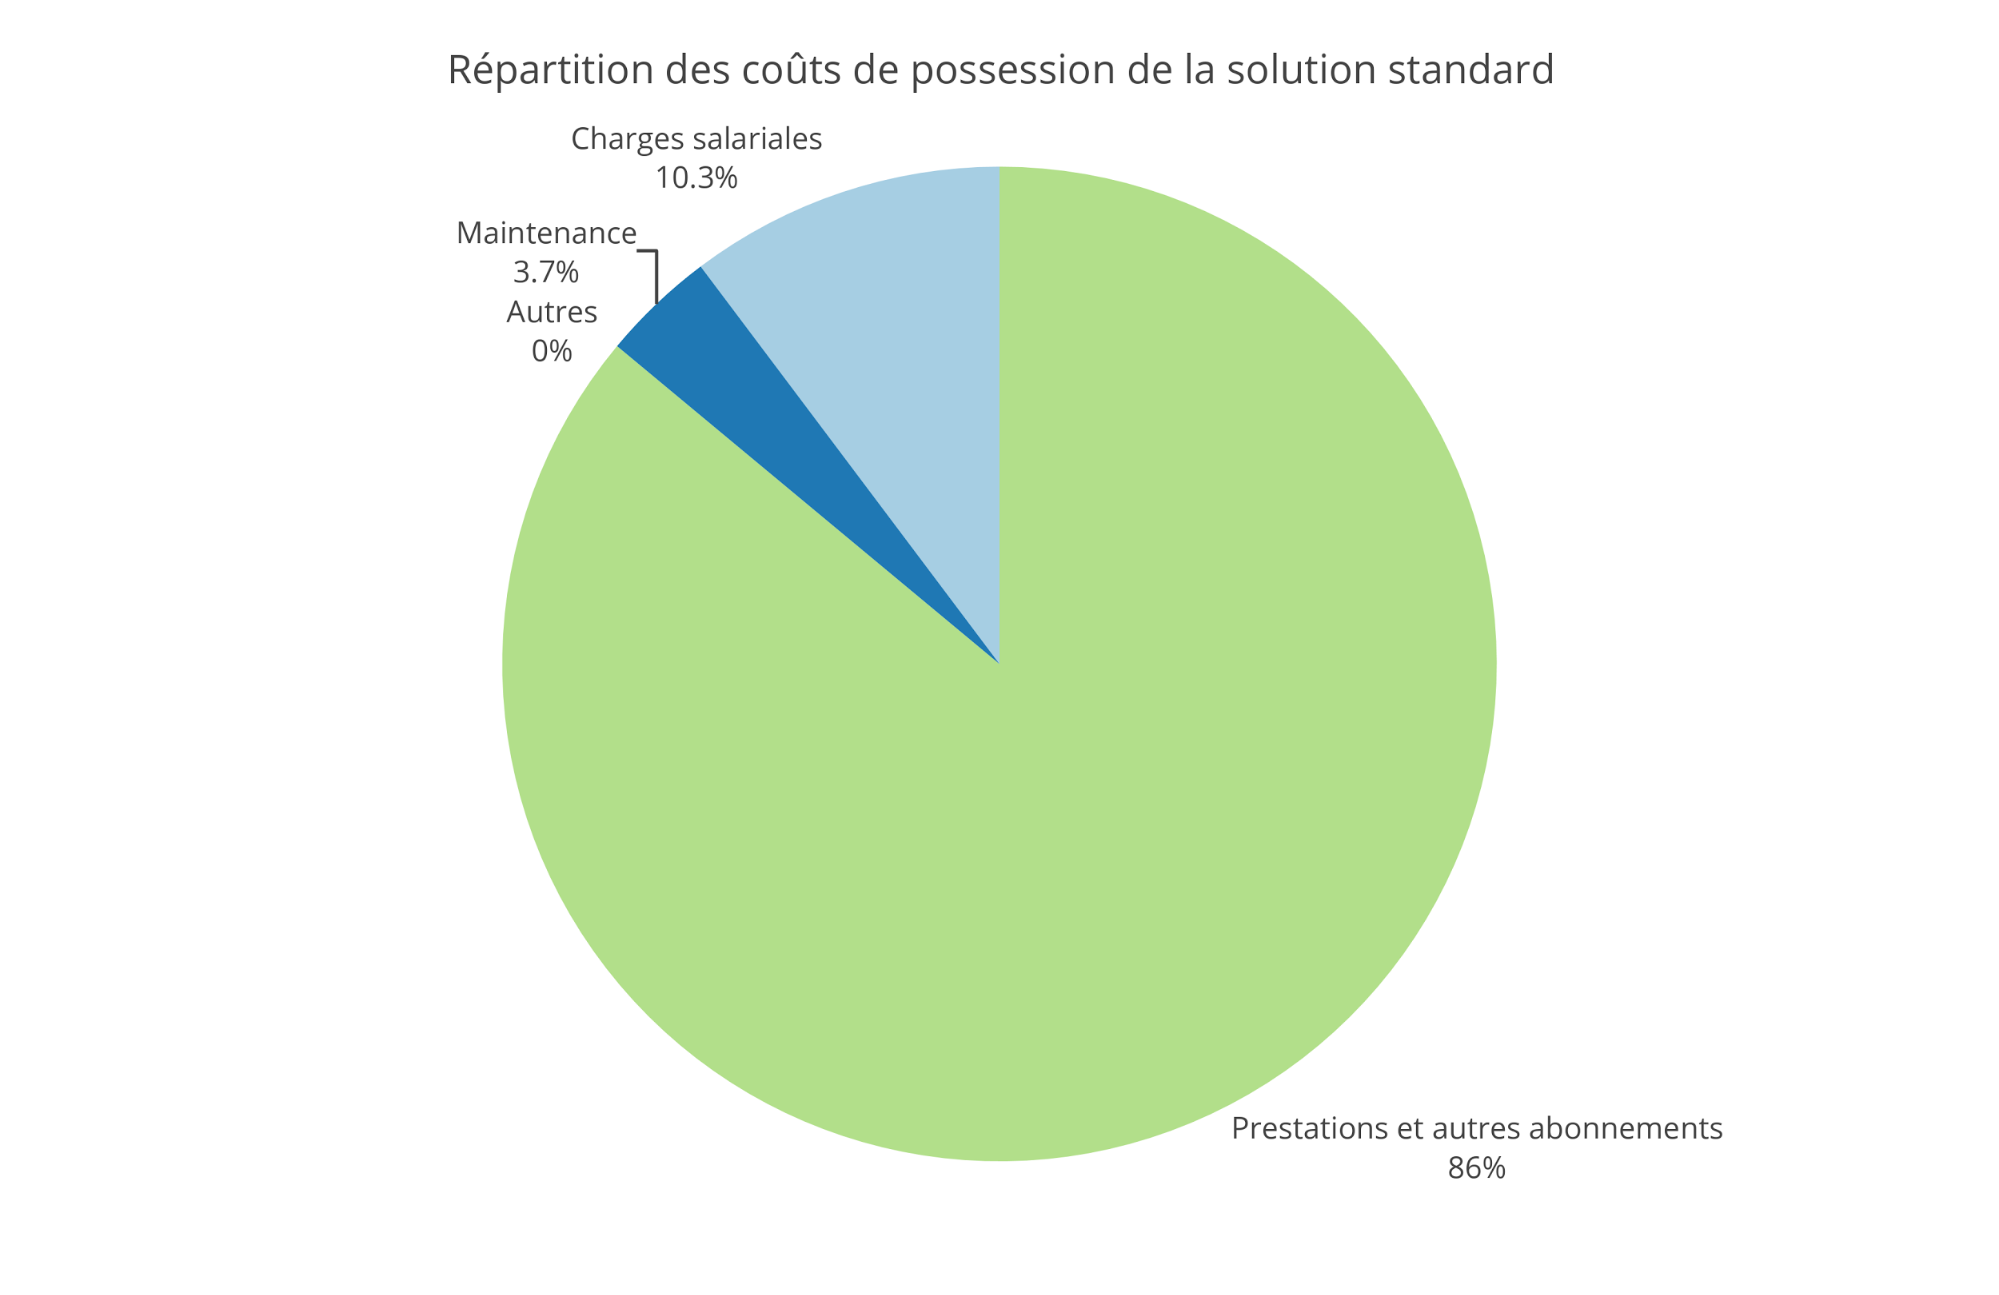
\includegraphics[width=12cm]{figures/cout_possession_sol_standard.png}}
\end{figure}


\section{Retour sur investissement (gains)}

\begin{shaded}
\noindent\textsc{Note :} 

Voir Annexe A pour le tableau d'évaluation.
\end{shaded}

Cette solution permettrait de nombreuses améliorations au sein du fonctionnement de l’entreprise. En effet, en passant par une solution standard, les coûts de maintenance sont fortement réduits. Cette réduction a un impact à la fois sur la maintenance logicielle et d’infrastructure. Des économies sont ainsi réalisées sur la réduction du nombre de jours de développement nécessaires et sur la réduction du nombre de jours soumis aux pannes matérielles, logicielles et réseau. De plus, grâce à la mise à disposition d’une plateforme optimisée et un suivi des processus amélioré, la productivité des employés s’en trouve grandement améliorée, permettant ainsi d’estimer de potentiels gains annuels. \\

En considérant la somme des gains réalisée chaque année grâce à cette solution standard et en intégrant les coûts de possession annuels, nous obtenons un retour sur investissement de 435 752 euros, par an. Ce retour sur investissement permet de rendre cette solution rentable en 10 mois, après sa mise en place.

\section{Évaluation des autres critères de comparaison}

Le fait d’utiliser la solution standard présente d’autres avantages. En effet, la solution sera déployée très rapidement et une transition plus rapide est possible. Il est bien connu que les périodes de transition ne sont pas favorables à une meilleure productivité. C’est dans ce cadre là que la solution standard a un atout certain car pas d’attente de réalisation très longue.

SAP est également pensé pour l’évotutivité et permet une rétrocompatibilité forte. C’est un avantage certains par rapport à d’autres ERP que l’on trouve sur le marché. Ainsi, par exemple l’ERP open-source \bf{odoo} peut demander une mise à jour complète de la base de donnée lors d’un changement de version.

On peut également supposer que de part l’importante utilisation de SAP dans le monde, la sécurité du logiciel est assez bien conçue. Cependant des recherches sur des moteurs de recherches en ligne avec pour mots clefs “failles SAP” montrent que le logiciel est quand même assez souvent victime de failles et de bugs. Ceci est également un des défauts de sa large utilisation. En effet, plus un logiciel est utilisé et plus il peut très intéressant de trouver de d’exploiter d’éventuelles failles.

La dernière chose à souligner dans  le cas de la solution standard est l’installation. Celle-ci n’est pas forcément aisée à faire manuellement. De ce fait il faudra l’intervention d’un consultant SAP pour l’installation, ainsi éventuellement d’un consultant de PeopleSoft de manière à ce que les différents logiciels interagissent correctement.

\part{Solution Spécifique}
\setcounter{section}{0}
\section{Rappel des fonctionnalités de la solution informatique et organisationnelle}

La solution spécifique est une solution développée spécialement pour l’entreprise. Elle ne repose pas en tout ou partie, contrairement à la solution standard, sur un progiciel déjà existant face auquel elle devra adapter ses processus. Ici, c’est la solution qui s’adapte à l’entreprise. \\

L’intégralité du logiciel doit donc être réalisé via des développements spécifiques, ainsi que les développements évolutifs ultérieurs à la mise en place de la solution. Il faut donc prévoir une équipe pour réaliser ce développement, qu’il soit interne ou sous traité.

\section{Chiffrages des coûts (d'acquisition et de possession)}

\begin{shaded}
\noindent\textsc{Note :}

    Voir Annexe B pour le tableau d'évaluation.
\end{shaded}

La mise en place d’une solution spécifique nécessite des investissements initiaux conséquents, qui correspondent en majeur partie à des immobilisations corporelles, basées sur du matériel informatique, à des immobilisations incorporelles, basées sur des licences logicielles et à des coûts de développement qui interviennent lors du déploiement du projet. L’important nombre de coûts d’acquisition découle sur un montant fort important d’investissement.

Les coûts de possession associés à la solution spécifique sont également fort important, les coûts de maintenance étant notamment élevés, ces derniers correspondant à 12\% des investissements initiaux. Les charges salariales correspondant aux nouveaux postes en charge de la gestion des nouveaux éléments du système d’information correspondent également à une augmentation de ces coûts de possession.

\begin{figure}[H]
    \noindent\makebox[\textwidth]{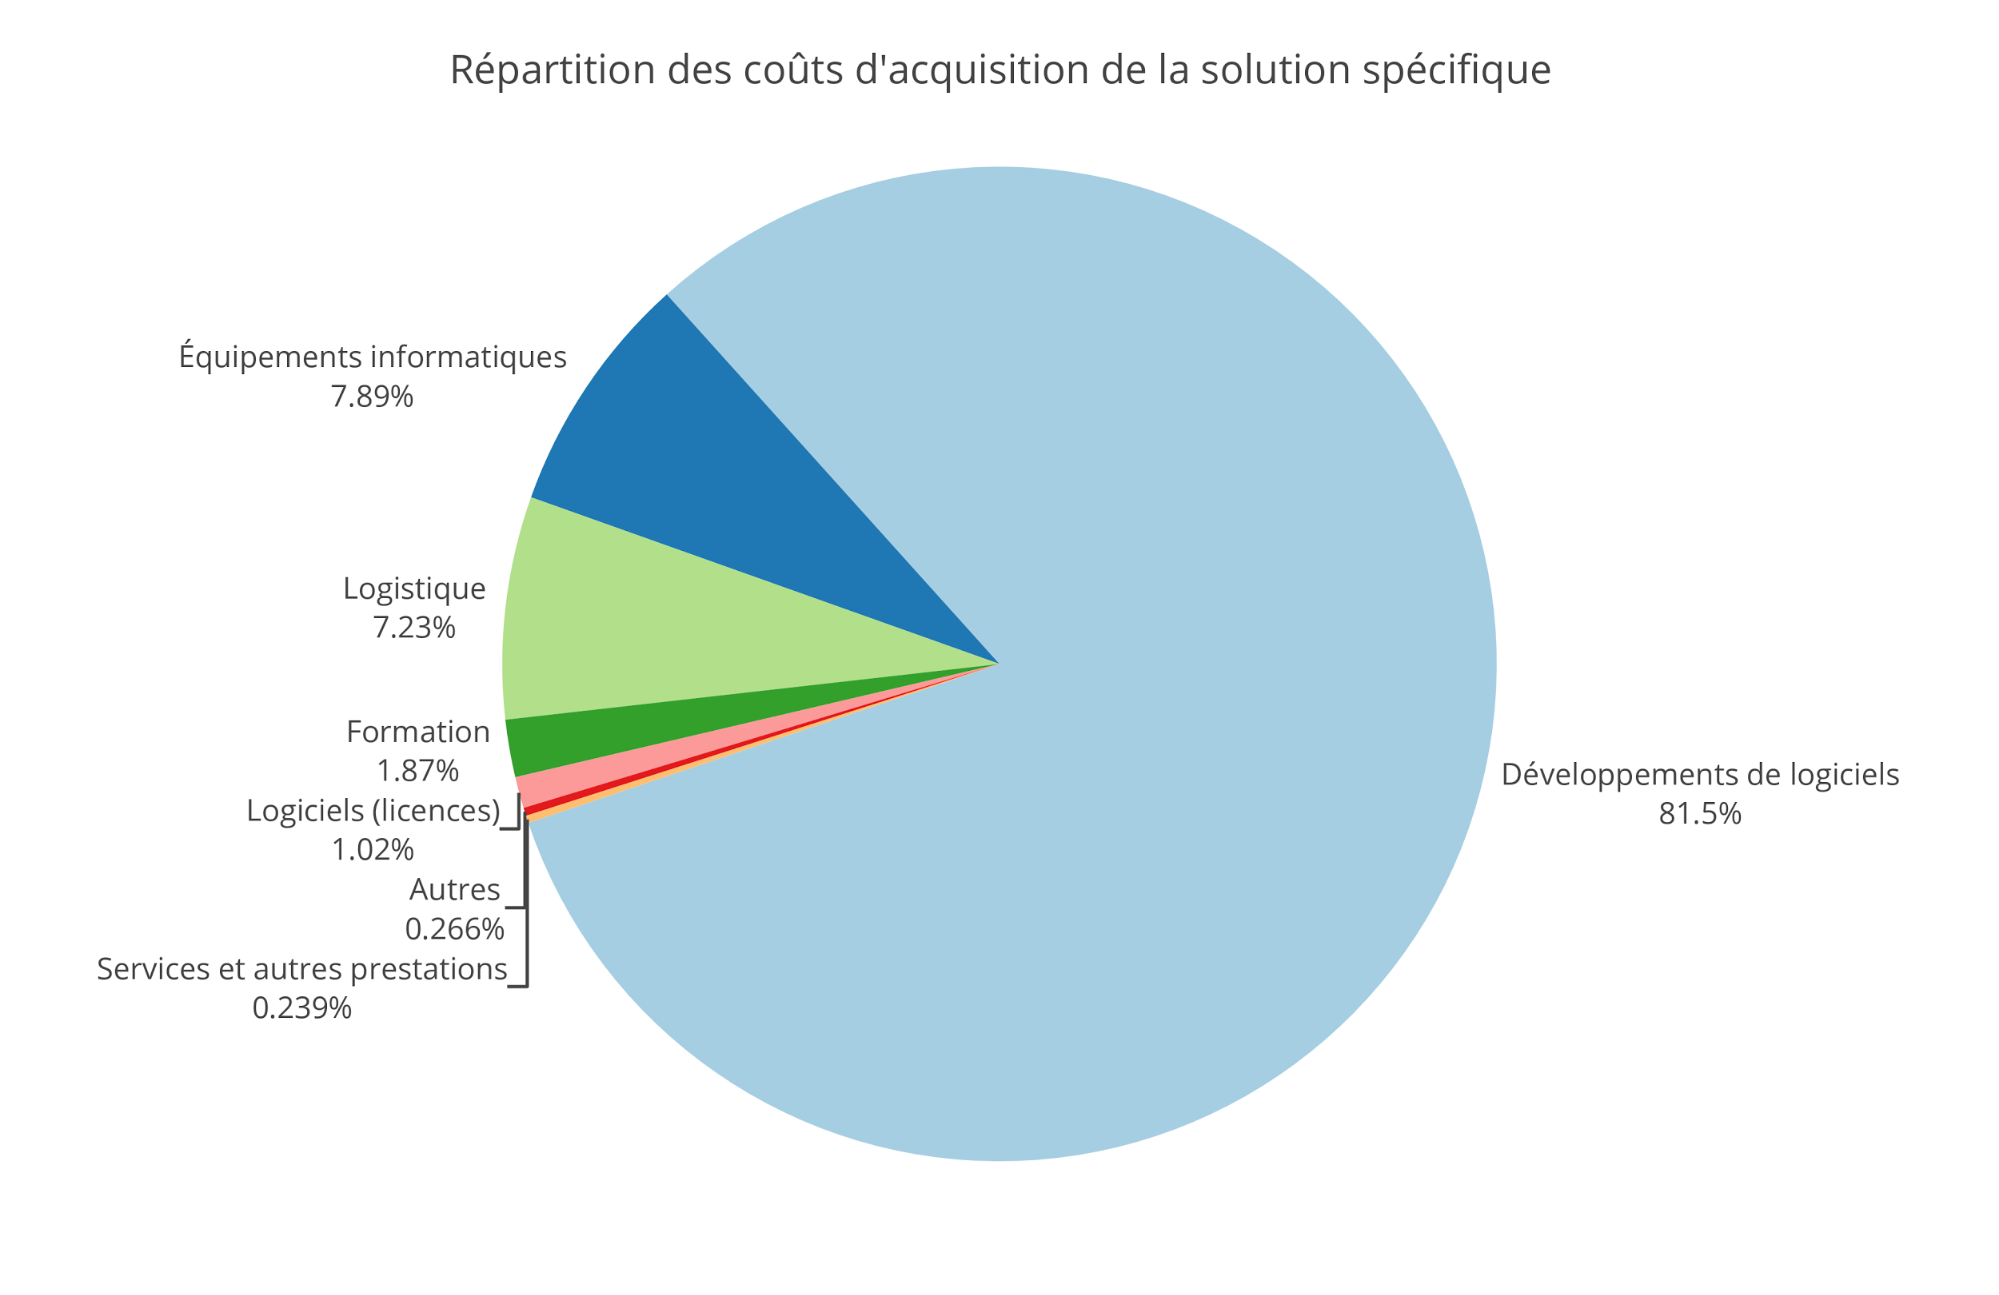
\includegraphics[width=12cm]{figures/cout_acquisition_sol_specifique.png}}
\end{figure}

\begin{figure}[H]
    \noindent\makebox[\textwidth]{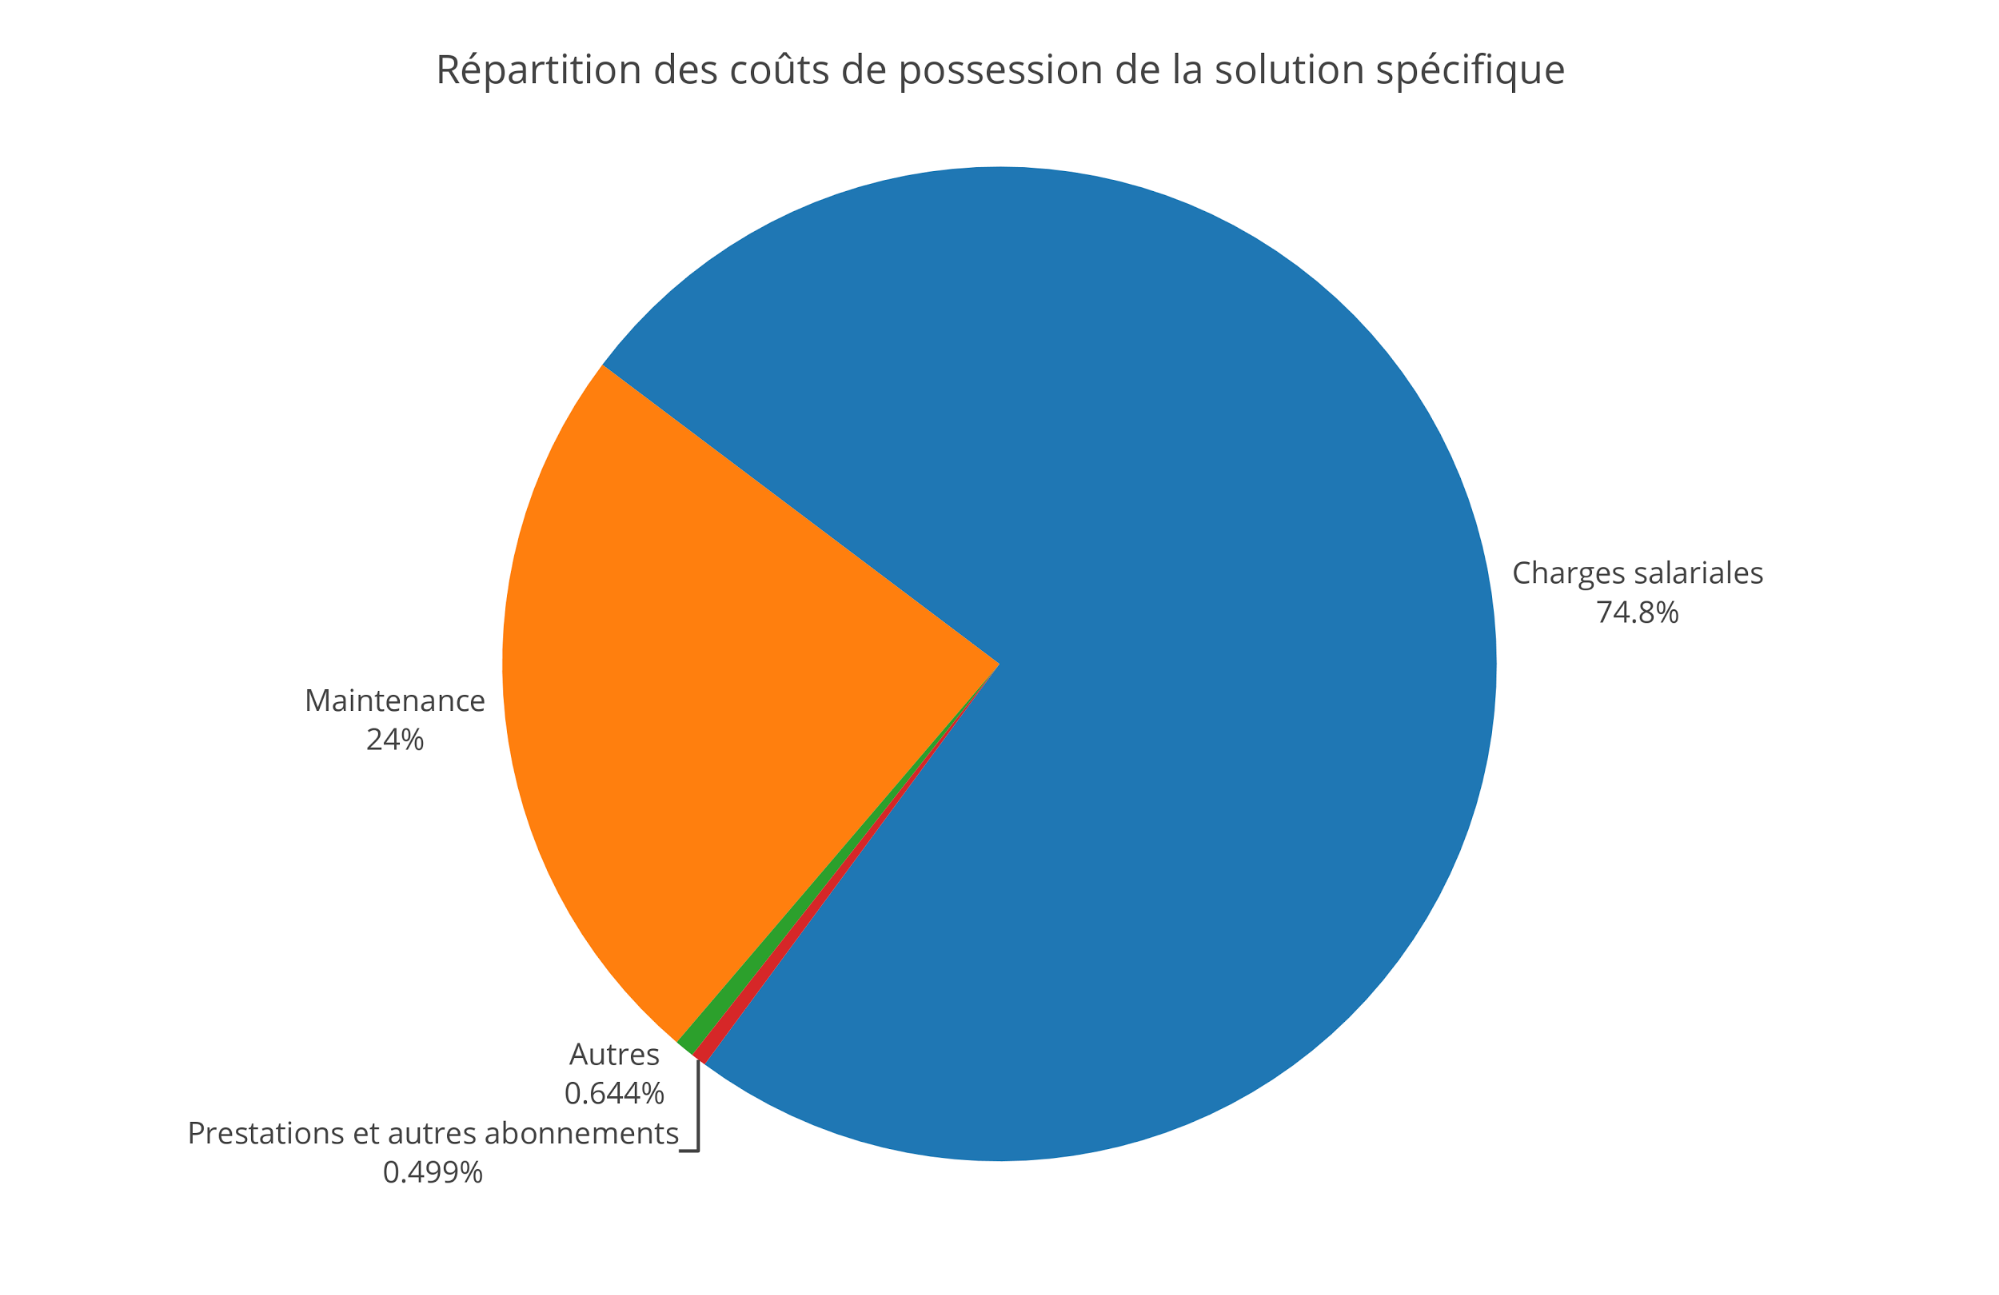
\includegraphics[width=12cm]{figures/cout_possession_sol_specifique.png}}
\end{figure}

\section{Retour sur investissement (gains)}

\begin{shaded}
\noindent\textsc{Note :}

    Voir Annexe B pour le tableau d'évaluation.
\end{shaded}

Le retour sur investissement de la solution spécifique est plus important, celui-ci s’élevant à 594 762,13 euros par an. En effet, la mise en place d’une solution sur mesure aux besoins de SPIE Sud-Est favorise grandement l’amélioration de la productivité de ses acteurs, sans pour autant bouleverser leurs habitudes de travail. Ainsi, la productivité des employés est augmentée, et les indicateurs mis en place permettent de réduire les risques tout en augmentant les performances réalisées par l’entreprise, expliquant ainsi le bon niveau de gain annuel, lié aux investissements réalisés en amont. \\

Cependant, étant donné l’importance des investissements ayant du être réalisés afin de mettre en oeuvre cette solution spécifique, celle-ci présente un délai de retour sur investissement de 24 mois, qui est plus long que celui proposé par la mise en place de la solution standard, avec toutefois un meilleur taux de retour sur investissement sur le long terme.

\section{Évaluation des autres critères de comparaison}

La solution est plus facile à faire évoluer et permet des développements spécifiques pour améliorer ou faire évoluer la solution. \\

A priori, elle permettra de ne pas trop modifier la structure du SI de l’entreprise. Ensuite, elle premettra de ne pas trop destabiliser les collaborateurs de SPIE en offrant une interface qui sera plus cohérente avec le reste de leur applications. \\

La sécurité de l’application sera dépendante de la sécurité générale des serveurs de SPIE, nous ne pouvons pas nous prononcer donc trop sur ce point. En revanche la fiabilité sera peut être moins bien car elle sera basée sur les anciens processus de SPIE, parfois peut adaptées. \\

L’évolution sera beaucoup plus simple que dans le cas de SAP étant donnée qu’elle sera interne à SPIE.

\part{Comparatif des solution}
\setcounter{section}{0}

Nous pouvons comparer les différents critères d’évaluation entre les deux solutions, afin d’identifier les avantages et inconvénients des solutions respectives. Cela permet par la suite d’adapter le choix de la solution aux besoins techniques et de mise en oeuvre de SPIE Sud-Est. Ainsi, nous pouvons remarquer dans le tableau ci-dessous que la solution spécifique dispose d’un score plus élevé que la solution standard, de façon générale. Cependant, ce score élevé requiert tout de même un fort investissement initial, des recommandations à prendre en compte sur le choix de la solution étant explicités dans le paragraphe suivant.

\begin{table}[H]
    \begin{tabular}{p{6cm}|p{2cm}|p{2cm}|p{3cm}|p{2cm}}
    Critère                             & \multicolumn{2}{l}{Solution standard} & \multicolumn{2}{l}{Solution spécifique} \\ \hline
    ~                                   & Évaluation & Score   & Évaluation   & Score   \\ \hline
    Mise en oeuvre                         & ~       & \bf{11} & ~            & \bf{14} \\ \hline
    Délai de mise en oeuvre                & 5 mois  & \bf{2}  & 12 mois      & \bf{1}  \\
    Délai d'adaptation au nouveau SI       & 1 mois  & \bf{4}  & 4 mois       & \bf{1}  \\ \hline
    Impact sur l'organisation              & ~       & \bf{4}  & ~            & \bf{9}  \\ \hline
    \it{Des structures}                    & Faible  & 1       & Moyen        & 2       \\
    \it{Des processus}                     & Moyen   & 2       & Léger        & 1       \\
    \it{De la relation partenaire}         & Faible  & 1       & Très positif & 3       \\ \hline
    Risques de mise en oeuvre              & Fort    & \bf{1}  & Faible       & \bf{3}  \\ \hline
    Critères techniques                    & ~       & \bf{6}  & ~            & \bf{10} \\ \hline
    Facilité d'intégration dans le SI      & Moyen   & \bf{1}  & Moyen        & \bf{1}  \\
    Adéquation aux besoins fonctionnels    & Bien    & \bf{1}  & Optimale     & \bf{3}  \\ \hline
    Qualités techniques                    & ~       & \bf{4}  & ~            & \bf{6}  \\ \hline
    \it{Fiabilité, sécurité}               & Moyen   & 2       & Faible       & \bf{1}  \\
    \it{Évolutivité, facilité de Maj}      & Bien    & 1       & Optimale     & \bf{3}  \\
    \it{Facilité d'utilisation, ergonomie} & Bien    & 1       & Moyenne      & \bf{2}  \\
    \end{tabular}
\end{table}

\part{Recommandations}
\setcounter{section}{0}

\todo{Compléter cette partie}

%% Inclure une figure :
%\begin{figure}[H]
%    \label{fig-LABEL-DE-LA-FIGURE}
%    \noindent\makebox[\textwidth]{\includegraphics[width=10cm]{figures/NOM-DE-LA-FIGURE.png}}
%    \caption{TEXTE DE LA LEGENDE}
%\end{figure}

%%% End document
\end{document}
